%# -*- coding: utf-8-unix -*-
%%==================================================
%% introduction.tex for seuthesis Bachelor Thesis
%%==================================================

\chapter{前言}
\emph{在泛函分析中,卷积、旋积或摺积(英语:Convolution)是通过两个函数f 和g 生成第三个函数的一种数学算子,表征函数f 与g经过翻转和平移的重叠部分的面积。}

\section{数学公式}
\subsection{简单的数学公式}
\textbf{卷积}(\textbf{convolution})在图像分析的线性方法中是一种重要的运算。卷积是一个积分,反映一个函数$f(t)$在另一个函数上$h(t)$移动时所重叠的量。函数$f$和$h$在有限域$[0,t]$上的$1D$卷积$f*h$由下式给出:
 $$(f*h)(t) \equiv \int_0^t {f(\tau )h(t - \tau )d\tau } $$

\subsection{带自动编号的公式}
这里可以限定在$[0,t]$区间,原因是我们假设负坐标部分的值是0。为了准确起见,我们还可以将卷积积分的上限扩展为$( - \infty ,\infty )$:
\begin{equation}(f*h)(t) \equiv \int_{ - \infty }^\infty  {f(\tau )h(t - \tau )d\tau }  = \int_{ - \infty }^\infty  {f(t - \tau )h(\tau )d\tau }
  \end{equation} 

\subsection{带等号对齐的公式}
卷积可以推广到更高维。令$2D$函数$f$和$h$的卷积$g$记为$f*h$,则有:
\begin{equation}
\begin{aligned}
(f*h)(x,y) &= \int_{ - \infty }^\infty  {\int_{ - \infty }^\infty  {f(a,b)h(x - a,y - b)} } dadb\\
 &= \int_{ - \infty }^\infty  {\int_{ - \infty }^\infty  {f(x - a,y - b)h(a,b)} } dadb\\
\end{aligned}
\end{equation}

\section{伪代码}
在写论文的时候我们通常要写伪代码,伪代码里面有时甚至还要包含数学公式(如根号一类的)。伪代码会自动找一个比较好的位置插入图片。

\begin{algorithm}
    \caption{用归并排序求逆序数}
    \begin{algorithmic}[1] %每行显示行号
        \Require $Array$数组,$n$数组大小
        \Ensure 逆序数
        \Function {MergerSort}{$Array, left, right$}
            \State $result \gets 0$
            \If {$left < right$}
                \State $middle \gets (left + right) / 2$
                \State $result \gets result +$ \Call{MergerSort}{$Array, left, middle$}
                \State $result \gets result +$ \Call{MergerSort}{$Array, middle, right$}
                \State $result \gets result +$ \Call{Merger}{$Array,left,middle,right$}
            \EndIf
            \State \Return{$result$}
        \EndFunction
        \State
        \Function{Merger}{$Array, left, middle, right$}
            \State $i\gets left$
            \State $j\gets middle$
            \State $k\gets 0$
            \State $result \gets 0$
            \While{$i<middle$ \textbf{and} $j<right$}
                \If{$Array[i]<Array[j]$}
                    \State $B[k++]\gets Array[i++]$
                \Else
                    \State $B[k++] \gets Array[j++]$
                    \State $result \gets result + (middle - i)$
                \EndIf
            \EndWhile
            \While{$i<middle$}
                \State $B[k++] \gets Array[i++]$
            \EndWhile
            \While{$j<right$}
                \State $B[k++] \gets Array[j++]$
            \EndWhile
            \For{$i = 0 \to k-1$}
                \State $Array[left + i] \gets B[i]$
            \EndFor
            \State \Return{$result$}
        \EndFunction
    \end{algorithmic}
\end{algorithm}

\section{插入图片}
在使用该命令的时候,图片会自动找一个他觉得比较好的位置插入图片,我们就不需要担心前面改了文字之后后面的格式乱掉。
\begin{figure}[htbp!]
\centering 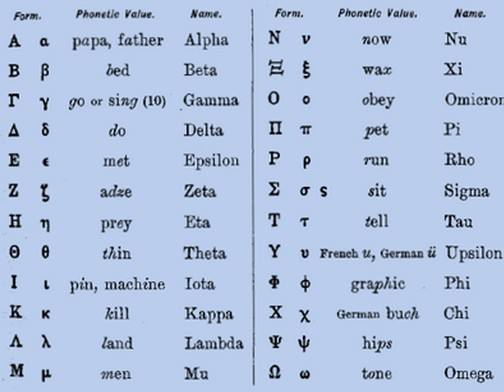
\includegraphics[width=0.9\textwidth]{img/test.jpg} \caption{图片的一个简单应用场景}
\end{figure}

\begin{figure}
\centering
\subfigure[the first subfigure]{
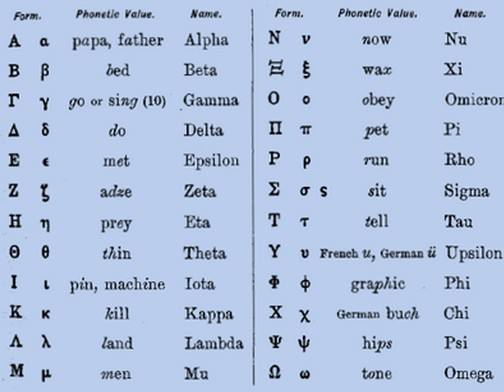
\includegraphics[width=0.4\textwidth]{img/test.jpg} 
}
\subfigure[the second subfigure]{
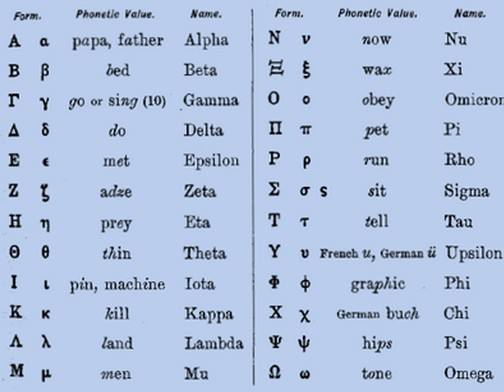
\includegraphics[width=0.4\textwidth]{img/test.jpg} 
}
\caption{子图应用场景}
\end{figure}

\section{引用论文}
使得论文符合要求\cite{Yao:2015ix}\cite{seucover}\cite{test1}\cite{test}\cite{R1}。